% DRAFT, written by Claude (AI) for the researcher to review and edit.
% Every number is traced in paper/notes.md. Sections marked [PLACEHOLDER]
% wait for the full cloud run. Do not submit before the researcher has
% rewritten and checked it.
\documentclass[11pt]{article}
\usepackage[utf8]{inputenc}
\usepackage[T1]{fontenc}
\usepackage{amsmath,amssymb}
\usepackage{graphicx}
\usepackage{booktabs}
\usepackage{xcolor}
\usepackage[margin=2.5cm]{geometry}
\usepackage[round,authoryear]{natbib}
\usepackage[hidelinks]{hyperref}
\newcommand{\placeholder}[1]{\textcolor{red}{[PLACEHOLDER: #1]}}
\newcommand{\pilot}[1]{\textcolor{blue}{#1}}

\title{An open, uniform machine-learning earthquake catalogue for central Mongolia from the 2012--2016 Central Mongolia Seismic Experiment (FDSN network XL)}
\author{[AUTHORS --- TBD]}
\date{Draft, \today}

\begin{document}
\maketitle

\begin{abstract}
\placeholder{Write after the full run. Planned structure: (1) the data gap for Mongolian microseismicity; (2) the pipeline (SeisBench ensemble picking, PyOcto, absolute location, waveform cross-correlation and GrowClust relocation, local magnitude, template matching); (3) event count, magnitude of completeness and location precision per subarray; (4) the seismogenic-depth and b-value comparison between the Hangay Dome, the Khövsgöl rift and the Gobi-Altai; (5) data and code availability.}
\end{abstract}

%=====================================================================
\section{Introduction}

Mongolia is one of the most seismically active continental interiors on Earth. Four earthquakes of magnitude about 8 struck the country in the first half of the twentieth century, including the 1905 Tsetserleg and Bulnay events \citep{schlupp2007,choi2018}, more than 2,000~km north of the India--Asia collision front. Present-day deformation is still measurable geodetically: GPS gives slip of a few mm/yr on the Bulnay fault and opening of about 4~mm/yr across the Baikal rift \citep{calais2003}. Microseismicity is the most direct way to see which of these faults are active today, at what depths the crust is brittle, and how earthquake sizes are distributed. It is also an input to seismic hazard models.

Yet the microseismicity of central Mongolia is poorly documented in open data. The Mongolian national network is registered with the International Federation of Digital Seismograph Networks (FDSN), but its waveforms are not openly distributed. In international bulletins the region is represented by only a few tens of events per year at magnitudes above about 3.5 (Section~\ref{sec:validation}). The best openly available record of small earthquakes is the Central Mongolia Seismic Experiment \citep[FDSN code XL;][]{xl_dataset,meltzer2019}. This US--Mongolian deployment of broadband seismometers ran from 2012 to 2016 in three subarrays: the Hangay Dome (HD, 2012--2014), the Khövsgöl rift (HV, 2014--2016) and the Gobi-Altai (AT, 2014--2016) (Figure~\ref{fig:stations}).

Several catalogues have been built from parts of XL, but none is public, uniform and complete. \citet{meltzer2019} described a preliminary catalogue for the Hangay subarray, built by automatic STA/LTA detection and association in Antelope followed by analyst review. It has a magnitude of completeness $M_c = 1.2$ (maximum curvature) and a $b$-value of 0.71, which the authors note ``could also reflect an incomplete earthquake catalog''. Its seismicity is restricted to the upper 20~km, with most events in the upper 10~km; the catalogue size was not reported and it was not released. Analysts of the Mongolian National Data Center hand-picked 12,912 events in the Hangay data from June 2012 to April 2014, and \citet{dashdondog2020} used 120 of them to derive a 1-D velocity model for the South Hangay; that catalogue is not public either. \citet{dashdondog2024,dashdondog2026} relocated subsets of Hangay events with HypoDD, and \citet{welkey2019} relocated the preliminary events in a preprint. For the Khövsgöl subarray, \citet{emanov2025} built an automated catalogue with the EQTransformer picker, grid-search association and Hypoinverse locations, and \citet{emanov2026} used it for depth sections. To our knowledge no catalogue of the Gobi-Altai subarray has been published. Machine-learning phase picks for the whole of XL are publicly available from the QuakeScope project \citep{ni2025}, but they are not associated into events.

Deep-learning phase pickers now routinely detect several times more earthquakes than energy-ratio detectors. Examples are PhaseNet \citep{zhu2019} and EQTransformer \citep{mousavi2020}, distributed with pretrained weights in SeisBench \citep{woollam2022}. Fast associators turn the resulting picks into catalogues \citep{zhu2022gamma,munchmeyer2024}. Essentially the same chain (PhaseNet, PyOcto, NonLinLoc and HypoDD) was recently applied to a 2023--2024 deployment at the Bulnay--Tsetserleg junction in Mongolia \citep{manceau2026,manceau2026data}. The method is therefore established in this region. What is missing is its uniform application to the whole XL dataset, with open data products.

Here we build, validate and release such a catalogue. We apply one pipeline, with identical parameters, to all three XL subarrays. It consists of an ensemble of six pretrained picker models, PyOcto association, absolute location, waveform cross-correlation and GrowClust relative relocation \citep{trugman2017}, local magnitudes, and template matching \citep{chamberlain2018,beauce2018}. A uniform catalogue allows a like-for-like comparison of seismogenic depth and $b$-value between a hot, elevated dome, a rift tip and a transpressional range, which has not been possible with the existing, method-specific catalogues. We test three hypotheses fixed before the full run (Section~\ref{sec:hypotheses}). \placeholder{one sentence on the main findings}

%=====================================================================
\section{Tectonic setting and data}
\label{sec:data}

\subsection{Setting}
The Hangay Dome is a broad, high plateau in central Mongolia, underlain by slow, hot upper mantle \citep{feng2021} and a conductive lower crust \citep{comeau2018}. Teleseismic waveform modelling indicates that earthquakes in Mongolia are confined to the upper $\sim$20~km. In the Baikal rift to the north, by contrast, they occur throughout the crust \citep{bayasgalan2005,deverchere2001}. Active strike-slip faults cross the apparently aseismic Hangay \citep{walker2008}. \citet{huang2022} proposed that a ring of strong lithosphere shields the dome interior from deformation. The Khövsgöl rift is the south-western end of the Baikal rift system, and the Gobi-Altai hosted the 1957 earthquake of magnitude about 8. Fault traces for interpretation come from the Active Faults of Eurasia Database \citep{zelenin2022}.

\subsection{Seismic data}
We use all broadband (HH, 100~Hz) channels of network XL \citep{xl_dataset}, obtained from the EarthScope Consortium FDSN web services. The station metadata list 114 station codes: 74 HD, 26 HV and 14 AT. Two HD codes operated only for a few weeks in 2012, leaving the 72 Hangay stations described by \citet{meltzer2019}. The station epochs sum to 75,267 station-days (48,187 HD, 17,602 HV, 9,478 AT), or about 1.3~TB of miniSEED (Figure~\ref{fig:availability}). Each station-day is downloaded, processed and deleted in a streaming pass (Section~\ref{sec:compute}). Only picks, a 20~Hz decimated copy for template matching and short event waveforms are kept.

\subsection{Reference catalogues}
For validation we use the ISC Bulletin \citep{isc_bulletin,storchak2017}, the EMSC and the USGS ComCat catalogues, retrieved through their FDSN event services. We also use the public QuakeScope PhaseNet picks for XL \citep{ni2025} and the published statistics of the preliminary Hangay catalogue \citep{meltzer2019}. Reference coverage is sparse. The ISC Bulletin contains 50 events in 43--50$^\circ$N, 94--105$^\circ$E during the whole Hangay deployment (10 June 2012 to 10 April 2014), EMSC contains 2 and ComCat 4.

%=====================================================================
\section{Methods}
\label{sec:methods}

\subsection{Ensemble phase picking}
We run two deep-learning pickers, PhaseNet \citep{zhu2019} and EQTransformer \citep{mousavi2020}, each with three sets of pretrained weights from SeisBench \citep{woollam2022}: weights trained on the global STEAD data set (\texttt{stead}), on the Italian INSTANCE data set (\texttt{instance}), and the authors' original release (\texttt{original}). That makes six model/weight pairs. Each pair is applied to the continuous, demeaned three-component day record, padded with 60~s from the neighbouring days. SeisBench's sliding-window stacking produces continuous P and S probability traces, and every probability peak above 0.2 is kept as a raw pick. Picking runs on GPU. On a benchmark station-day, picks computed on a GPU (Apple MPS backend) were identical to the CPU picks to within 10~ms (\pilot{11/11 PhaseNet and 14/14 EQTransformer picks}).

The ensemble merges raw picks per station and phase. Picks from different model/weight pairs within 0.3~s (P) or 0.5~s (S) of each other form a group, with at most one pick per pair. The ensemble pick time is the probability-weighted mean of the group, and its probability is the mean over all six pairs, counting a missing pair as zero. A group is kept if at least two pairs support it and its mean probability is at least 0.1. If a P and an S ensemble pick at one station fall within 0.5~s of each other, the less probable one is discarded. On the first two pilot days, a stricter threshold of 0.3 kept 3,265 picks and yielded 25 events. The adopted threshold kept 13,384 picks and yielded 44 events, including 96\% of the stricter set and several small events located with residuals below 0.2~s. The STEAD-trained weights rarely fire on these data, which makes a mean over all six pairs overly punitive at 0.3. \placeholder{confirm on the full pilot month}

\subsection{Association}
Ensemble picks are associated with PyOcto \citep{munchmeyer2024}. PyOcto searches the space--time volume of possible origins by recursive octree subdivision. It retains cells that can explain enough picks within a travel-time tolerance, given a 1-D velocity model. We use the eight-layer 1-D model that \citet{dashdondog2020} derived for the South Hangay from local earthquakes recorded by this array (Table~\ref{tab:vmodel}; $V_P/V_S \approx 1.73$, Moho at 50~km). As a robustness check, all events are also located in a two-layer model built from the average crustal velocities of \citet{meltzer2019}: $V_P = 6.4$~km/s and $V_S = 3.6$~km/s over a Moho at 50~km, with $8.0$ and $4.5$~km/s below. An event requires at least 8 picks, including at least 4 P picks and 2 S picks, and at least 2 stations with both phases. Travel times come from exact first-arrival tables (direct and head waves) computed for the layered model, written in PyOcto's table format. The association and the locator therefore use identical times. The travel-time tolerance is 1.5~s, and stations more than 300~km from a candidate origin do not count towards association. On the pilot data this cutoff left the events unchanged and made association 35--160 times faster. The search volume covers the station footprint plus a 100~km margin and depths of 0--60~km. Events within 0.2$^\circ$ of the volume edge are flagged as probably external. Large regional events are occasionally split into two associations, the second built from later regional phases. Of two events within 20~s and 150~km of each other, we therefore keep the one with more picks. On pilot days 1--2 this removed 4 of 44 events, each a duplicate of an ISC/BYKL event north-east of the array.

\subsection{Absolute location}
Each associated event is relocated with a weighted, robust (soft-$L_1$) least-squares inversion of its P and S arrival times for hypocentre and origin time. We start from the PyOcto solution and from several fixed starting depths to avoid local minima. Travel times are interpolated from the same first-arrival tables as used for association. Depths are relative to sea level and cannot be negative; station elevation enters as a vertical travel-time static. Pick weights are the ensemble probabilities, halved for S. Formal 1$\sigma$ uncertainties come from the scaled covariance matrix: horizontal (major semi-axis, $e_h$), depth ($e_z$) and origin time. Each event gets a quality class. Class A requires an rms residual $\le 0.5$~s, an azimuthal gap $\le 180^\circ$, $e_h \le 3$~km, $e_z \le 5$~km, a nearest station within $\max(15~\text{km}, 1.5\times\text{depth})$, and a depth not at a search bound. Class B requires rms $\le 0.8$~s, gap $\le 250^\circ$, $e_h \le 6$~km and $e_z \le 10$~km. Class C covers the remaining located events, and class D marks events with rms above 1~s or at the edge of the search volume. \placeholder{NonLinLoc probabilistic locations \citep{lomax2000} as a cross-check, if added}

\subsection{Local magnitude}
For each event we store three-component waveforms from every station with a pick and every station within 150~km. The window runs from 10~s before the predicted P arrival to 20~s after the predicted S arrival, and is at least 60~s long. Local magnitude $M_L$ uses the peak amplitude $A$ (mm) of each horizontal component after deconvolution to displacement and convolution with a Wood--Anderson response. That response has a natural period of 0.8~s, damping 0.7 and magnification 2080 \citep{uhrhammer1990}. The amplitude is measured from 1~s before P to 10~s after S. The distance correction is that of \citet{hutton1987}:
\begin{equation}
M_L = \log_{10} A + 1.110 \log_{10}(R/100) + 0.00189\,(R-100) + 3.0,
\end{equation}
where $R$ is the hypocentral distance in km. The event magnitude is the median over station-components, after station corrections (median residuals of stations with at least 10 readings). Its uncertainty is the scaled median absolute deviation. We check whether the station residuals trend with distance, as a test of the Southern-California attenuation term in Mongolia. \placeholder{decide whether to adopt the Mongolian $M_L$ scale of \citet{ganbat2026ml}, after reading it and comparing on the full catalogue}. A constant offset to the ISC/EMSC/USGS magnitudes of matched events is estimated with a bootstrap. The magnitude types differ ($m_b$, $M_L$, $M_w$), so we report the offset rather than force our scale onto theirs.

\subsection{Relative relocation}
Differential travel times come from waveform cross-correlation of every event pair within 10~km, keeping each event's 40 nearest neighbours. Waveforms are band-passed at 2--15~Hz. P windows on the vertical component span $-0.5$ to $+1.0$~s around the pick. S windows on both horizontals span $-0.5$ to $+2.0$~s, and the correlation functions of the two horizontals are averaged. The lag search is $\pm0.6$~s. Normalised correlation coefficients are computed as one batched grouped convolution in PyTorch \citep{paszke2019}, and lags are refined to sub-sample precision with a parabola. Pairs with $CC \ge 0.6$ are used. Events are relocated with GrowClust \citep{trugman2017} in the same primary 1-D model, with relative uncertainties from 100 bootstrap resamples.

\subsection{Template matching}
To lower the detection threshold, quality-A events recorded at six or more stations serve as templates in EQcorrscan \citep{chamberlain2018}. The cross-correlations run on the GPU through the fast\_matched\_filter backend \citep{beauce2018}. Templates are 4~s long, start 0.5~s before the pick, and use the 2--8~Hz band of the 20~Hz decimated data: P on the vertical, S on both horizontals. A detection is declared when the network-summed correlation exceeds 9 times its daily median absolute deviation, and detections within 2~s of each other are declustered. \placeholder{magnitudes of detections from amplitude ratios to the template; number of templates and detections}

\subsection{Catalogue statistics}
\label{sec:hypotheses}
The magnitude of completeness $M_c$ is estimated by maximum curvature with a $+0.2$ correction \citep{woessner2005} and by the goodness-of-fit method at 90 and 95\% \citep{wiemer2000}, with bootstrap uncertainties. $b$-values use the maximum-likelihood estimator \citep{aki1965} with the binning correction $M_c - \Delta M/2$ \citep{utsu1966}, the \citet{shi1982} standard error, and bootstrap 95\% intervals. Seismogenic depth is measured as $D_{90}$ and $D_{95}$, the depths above which 90 and 95\% of the events lie. They are computed from quality-A events, with bootstrap intervals, per region (Hangay interior, Hangay margin, Khövsgöl, Gobi-Altai). The region polygons were drawn before any depth or $b$-value was computed. Possible quarry blasts are flagged, not removed, by the day/night event-rate ratio in 0.25$^\circ$ cells, by local working hours and by shallow depth. The hypotheses, fixed before the full run, are:
H1, the Hangay $M_c$ of the ML catalogue is below 1.2, the value of \citet{meltzer2019};
H2a, $D_{90}$ is greater beneath Khövsgöl than beneath the Hangay;
H2b, $D_{90}$ is greater at the Hangay margins than in the dome interior;
H3, the Hangay $b$-value at our $M_c$ exceeds 0.71.
\placeholder{the researcher should confirm or freeze the hypotheses and regions (config/regions.geojson) before the full run}

\subsection{Computation}
\label{sec:compute}
The full run streams the data through one rented GPU (NVIDIA RTX 4090). Each station-day is downloaded with one FDSN request, picked by all six model/weight pairs, merged into ensemble picks, decimated to 20~Hz for template matching, and then deleted. A progress ledger makes every stage resumable. Pilot development used an Apple M4 laptop. \placeholder{measured wall-times per pass, and total cost}

%=====================================================================
\section{Validation of the method on a pilot month}
\label{sec:validation}
\placeholder{FILL FROM results/validation_month.md: January 2013, Hangay subarray, 72 stations.}

\subsection{Picks compared with QuakeScope}
Our PhaseNet run with the INSTANCE weights, at the QuakeScope threshold of 0.2, reproduces \pilot{96\%} of the QuakeScope XL picks on pilot days 1--2 (P 8,782 of 9,130; S 5,163 of 5,335) with zero median time difference. This identifies the QuakeScope model as PhaseNet/INSTANCE and verifies our data handling independently. We also reproduced exactly the published QuakeScope count for May 2013 (209,901 picks on 72 stations; \citealp{ni2025}). \placeholder{full-month numbers from results/quakescope\_pilot\_2013-01.md; events from associating QuakeScope picks with the same PyOcto settings (days 1--2: 45 events, versus 44 from our ensemble)}

\subsection{Events compared with ISC, EMSC and USGS}
\placeholder{from results/validation\_pilot\_2013-01\_refs.md}

\subsection{Comparison with the preliminary Hangay catalogue}
\placeholder{event rate per month compared with \citet{meltzer2019}}

%=====================================================================
\section{The catalogue}
\placeholder{FULL RUN: event counts per subarray, $M_c$ per subarray and through time, location uncertainties, Figure: seismicity map on AFEAD faults, Figure: frequency--magnitude distributions.}

\section{Fault activity}
\placeholder{FULL RUN: which AFEAD faults carry seismicity above $M_c$; along-strike profiles; Table of per-fault statistics.}

\section{Seismogenic depth and $b$-values}
\placeholder{FULL RUN: $D_{90}$/$D_{95}$ per region with bootstrap intervals (H2a, H2b); $b$-values (H3); comparison with \citet{emanov2026} for Khövsgöl and with \citet{dashdondog2026} for the Egiin Davaa fault.}

\section{Discussion}
\placeholder{Thermal interpretation (\citealp{comeau2018,feng2021}); the shielding hypothesis of \citet{huang2022}; comparison with the Khövsgöl catalogue of \citet{emanov2025}; limitations: 1-D velocity model and depth resolution, station spacing, the reference catalogues are sparse, the pretrained pickers were not fine-tuned on Mongolian data, magnitudes are calibrated with few reference events.}

\section{Conclusions}
\placeholder{4--5 numbered findings.}

%=====================================================================
\section*{Data and code availability}
Waveforms are from the Central Mongolia Seismic Experiment \citep[network XL, doi:10.7914/SN/XL\_2012;][]{xl_dataset}, accessed through the EarthScope Consortium FDSN web services. The code is at \url{https://github.com/brkh1222-byte/mongolia-quake-catalog}. \placeholder{Zenodo DOI for the catalogue (CSV + QuakeML), picks and code release.} The pipeline uses ObsPy \citep{beyreuther2010,krischer2015}, SeisBench, PyOcto, PyTorch, GrowClust, EQcorrscan and fast\_matched\_filter.

\section*{AI-use statement}
[AI-USE STATEMENT --- TBD]. \textit{Factual note for the researcher, to be turned into the statement:} the code, the analyses and this draft were produced by an AI assistant (Claude, Anthropic), directed by the researcher, who reviewed and edited the text. All references were checked against Crossref/DataCite records.

\section*{Acknowledgements}
\placeholder{XL PI and field teams (A. Meltzer, Lehigh University; Institute of Astronomy and Geophysics, Mongolian Academy of Sciences); EarthScope data services; QuakeScope.}

\section*{Competing interests}
The authors declare no competing interests.

\begin{table}[p]
\centering
\caption{Primary 1-D velocity model \citep[][their Table 1]{dashdondog2020}. Depths are layer tops relative to sea level.}
\label{tab:vmodel}
\begin{tabular}{rrr}
\toprule
Depth (km) & $V_P$ (km/s) & $V_S$ (km/s) \\
\midrule
$-5$ & 6.06 & 3.50 \\
14 & 6.16 & 3.50 \\
20 & 6.27 & 3.63 \\
25 & 6.36 & 3.68 \\
30 & 6.53 & 3.79 \\
35 & 6.63 & 3.91 \\
45 & 7.16 & 4.18 \\
50 & 8.00 & 4.62 \\
\bottomrule
\end{tabular}
\end{table}

%=====================================================================
\begin{figure}[p]
\centering
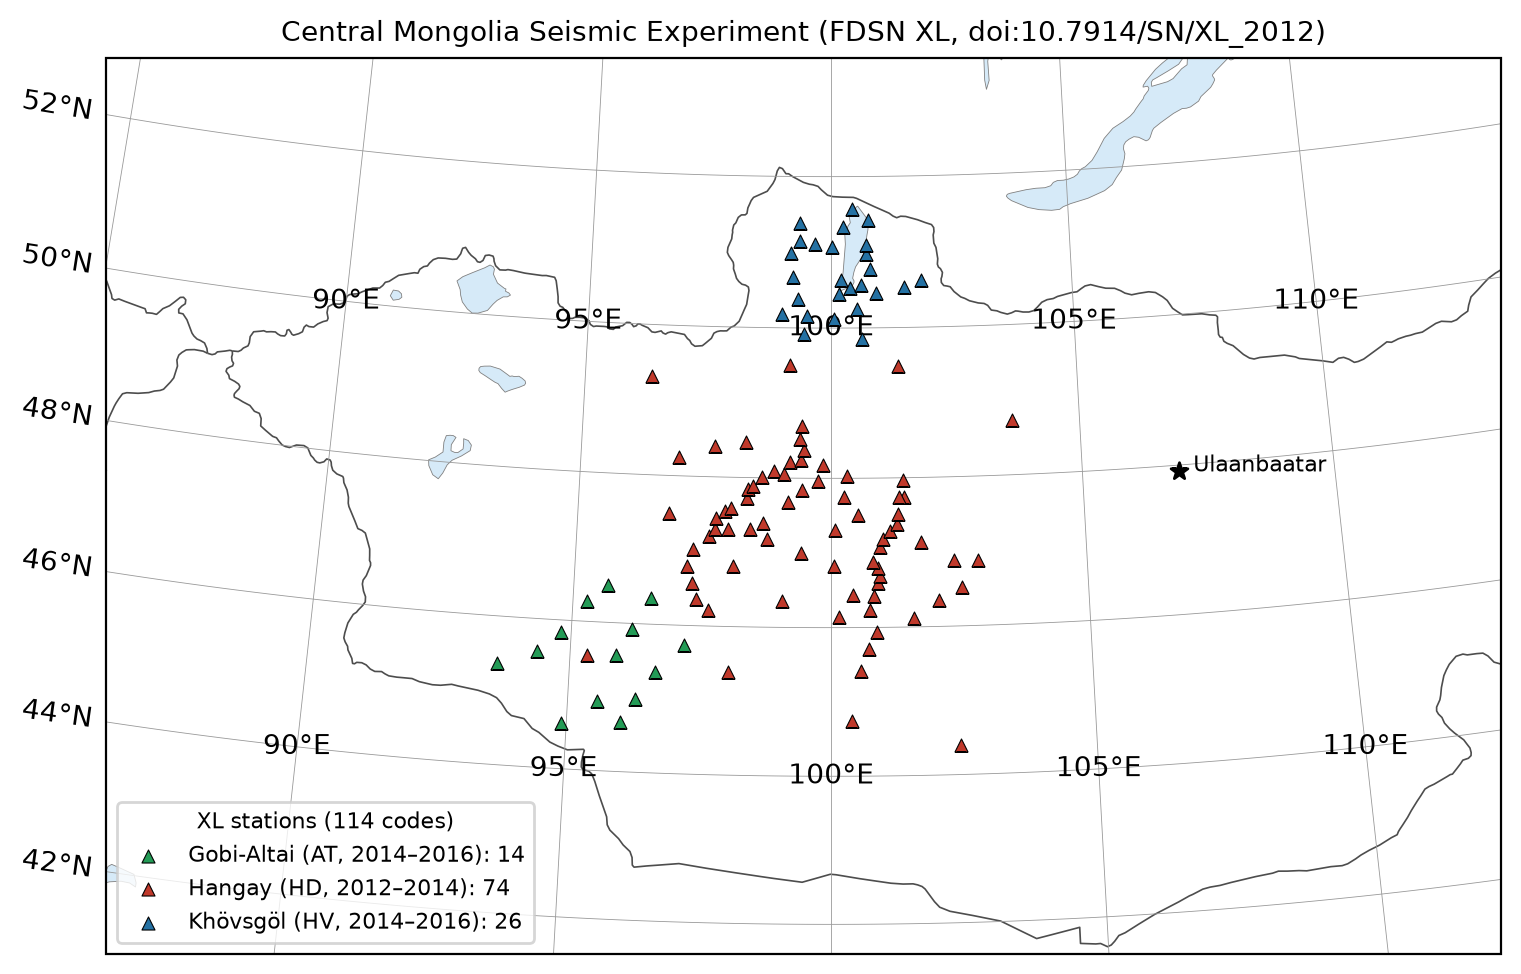
\includegraphics[width=0.85\textwidth]{../results/fig_stations.png}
\caption{Stations of the Central Mongolia Seismic Experiment (FDSN network XL), by subarray.}
\label{fig:stations}
\end{figure}

\begin{figure}[p]
\centering
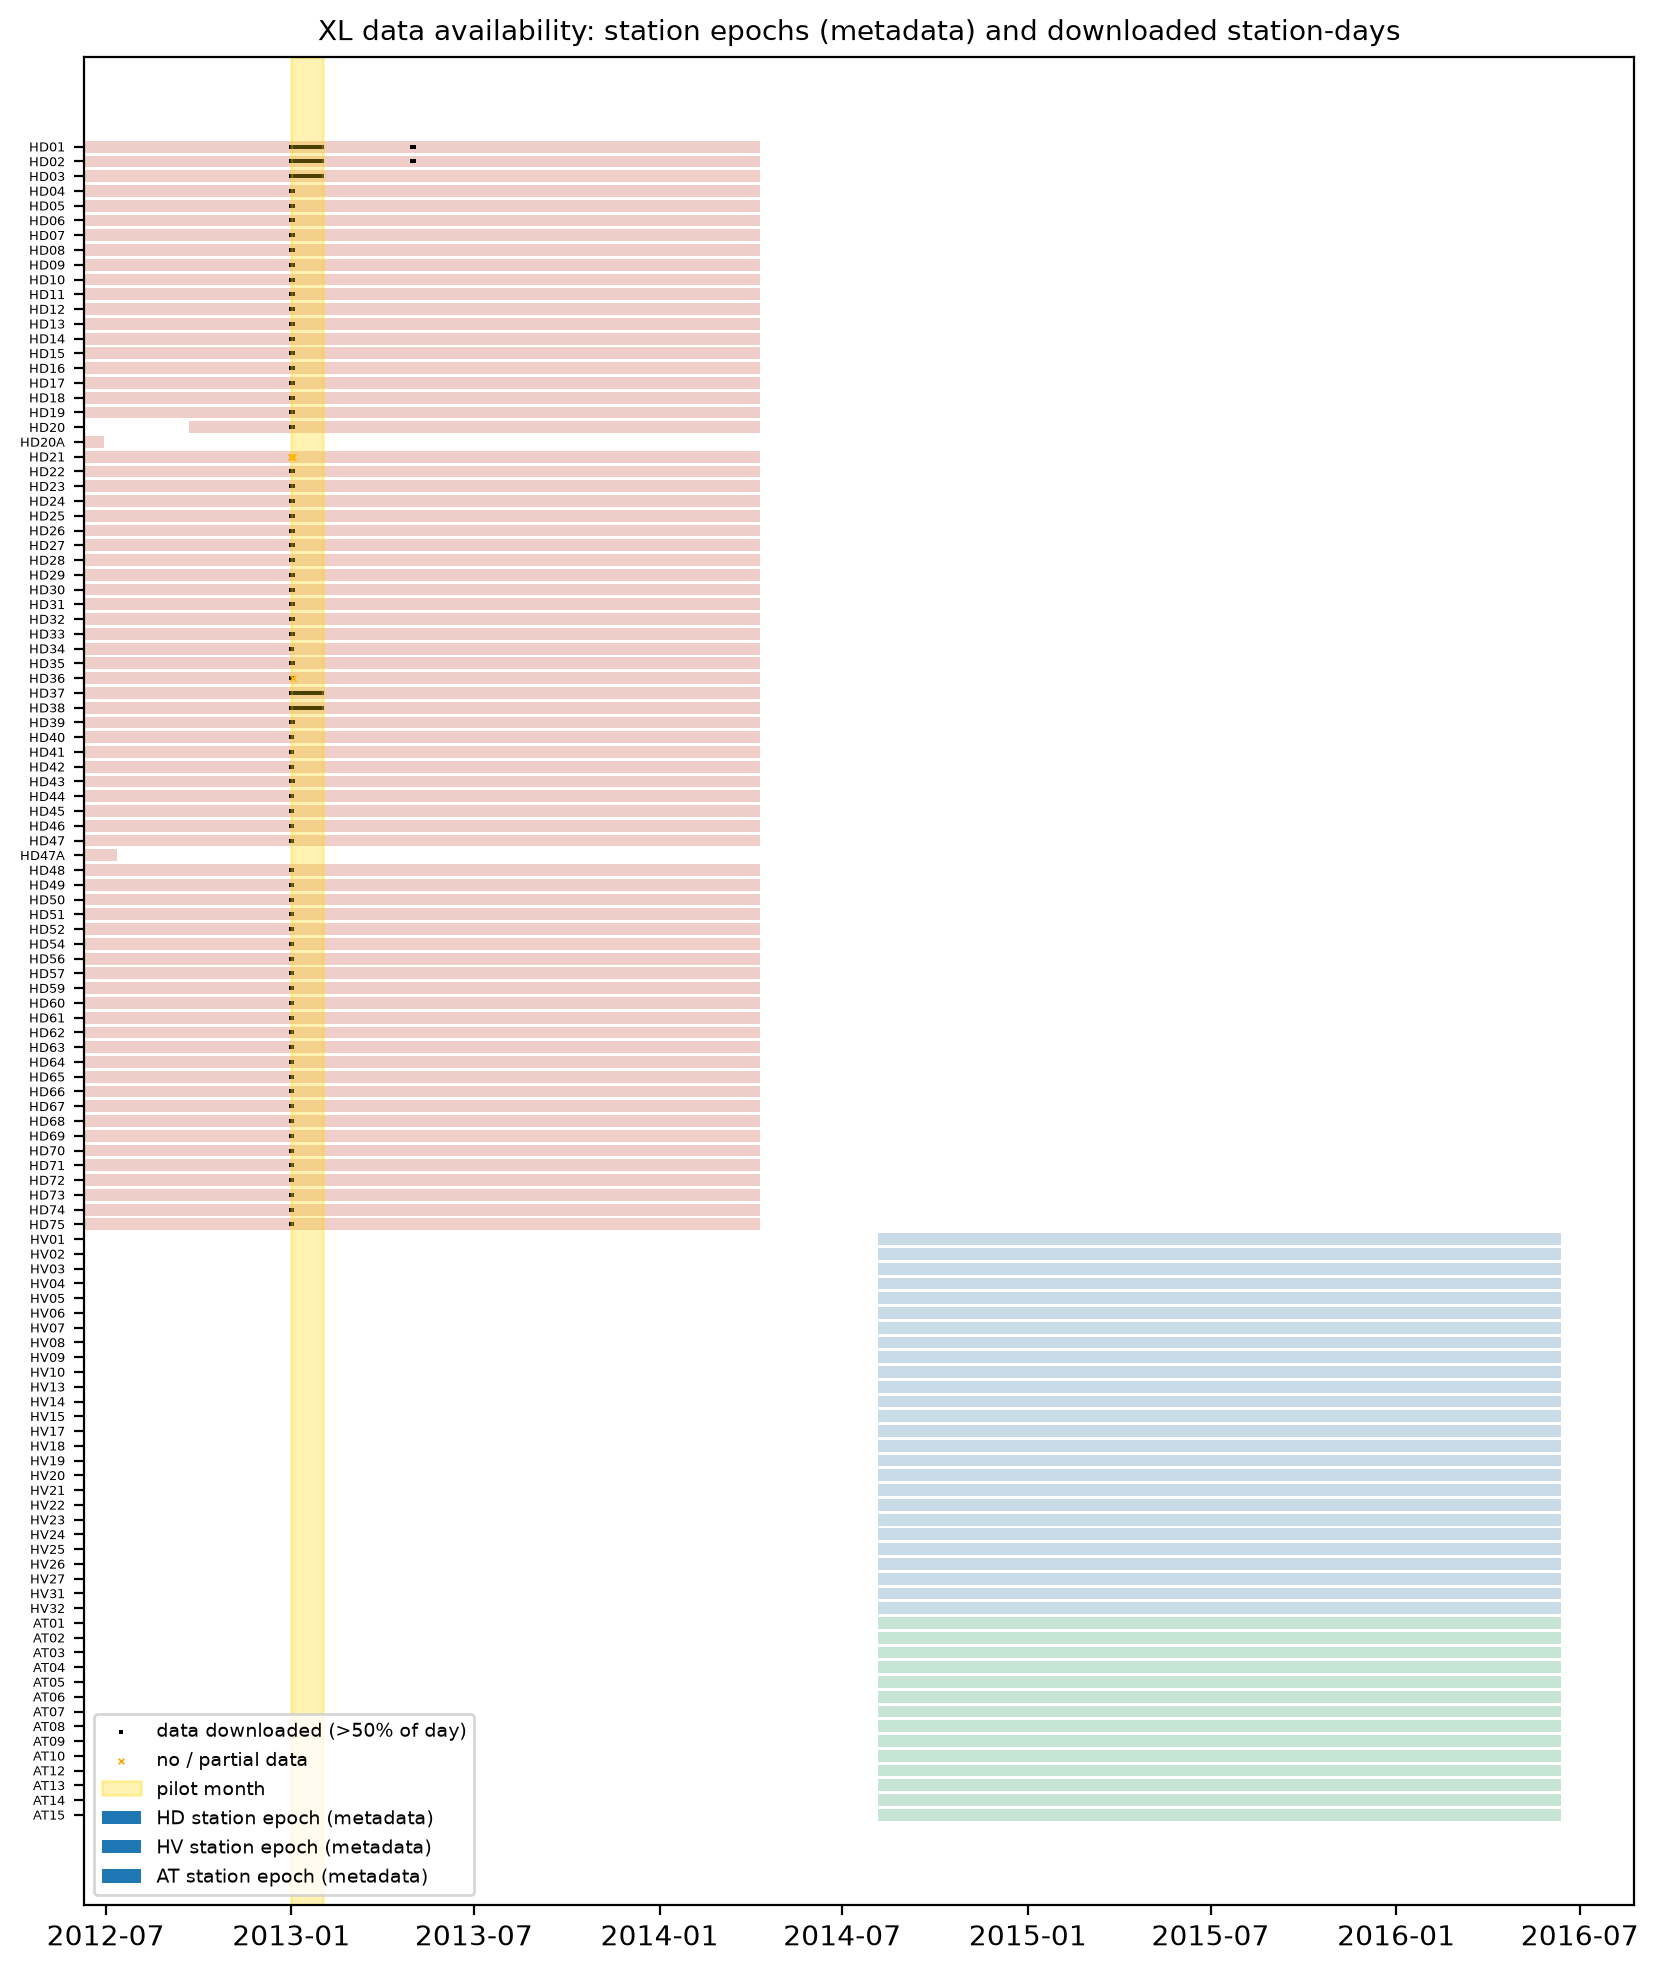
\includegraphics[width=0.95\textwidth]{../results/fig_availability.png}
\caption{Data availability per station from the station metadata (epochs), with the pilot month marked.}
\label{fig:availability}
\end{figure}

\bibliographystyle{plainnat}
\bibliography{references}
\end{document}
